\documentclass{article}

% Language setting
% Replace `english' with e.g. `spanish' to change the document language
\usepackage[english]{babel}

% Set page size and margins
% Replace `letterpaper' with `a4paper' for UK/EU standard size
\usepackage[letterpaper,top=2cm,bottom=2cm,left=3cm,right=3cm,marginparwidth=1.75cm]{geometry}

% Useful packages
\usepackage{amsmath}
\usepackage{graphicx}
\usepackage[colorlinks=true, allcolors=blue]{hyperref}

% Comment package for multi-line comments
\usepackage{comment}

\title{Concept Intelligent Agents Geomates Practicals}
\author{Ali Baran Oez, Mohammad Ghassan Aburas, Martin Stuwe, Jendrik Stoltz}

\begin{document}
\maketitle

\section{Main Idea}

The main Idea of our agent is the combination of planning systems and a Large Language Model (LLM) on different levels of control of the agent. 
With the capability of LLMs of handling loosely defined tasks, the LLM gets tasked to find sub-goals / critical points in the level and select one of them as the first goal. As communication is hard with unknown agents in the level,  the Theory of Mind capabilities of LLMs discussed in the lecture are expected to select actions that fit to what the other agent might do in the situation. 
In the proposed agent, the LLM acts as a black box learning element receiving a world description and returning a high level goal. We hope that the various types of background knowledge encoded in the weights in combination with in context learning will make the LLM propose sub-goals based on expected and observed behaviour of the other human or autonomous player and structure of the level.

Planning Systems on the other hand offer deterministic results and do not have the hallucination problem of LLMs in complex reasoning tasks ensuring correct plans for reaching goals. Planning systems also have a lower answer latency and are much lighter on resources than the inference of large neural networks. 

\section{Self Localization}

To select a possible set of actions for the used planning system and give the LLM a suitable task description, the agent has to learn wether it controls the ball or the rectangle first. Our self localization approach is inspired by the sense of control concept introduced in the perception in agents lecture. 
In the geometry friends game, the effect of key presses on the two different player types is defined in the task description.
Our agent will choose a random control key, and press it and observe the change on environment. 
To detect the change, a simple model of position and velocity of the two players is used. 
The actions and expected changes are organized as pairs for each of the different agent types.
To reduce the chance of the other player choosing the same action for their self localization procedure, the process is repeated multiple times (e.G. 8 times) like described in the pseudo code below. To determine the player type, the type with the higher sense of control is chosen. After determining the player type, the actual agent control code is started.

\begin{verbatim}
rect_soc = 0
disc_soc = 0
world_state_old = get_world_state()

repeat n times:
    key = select_random([W,A,S,D])
    exp_effect_rect = get_exp_effect(key, 'rect')
    exp_effect_disc = get_exp_effect(key, 'disc')
    press(key)
    world_state = get_world_state()
    rect_soc += check_effect(exp_effect_rect, world_state_old, world_state)
    disc_soc += check_effect(exp_effect_disc, world_state_old, world_state)
    world_state_old = world_state

\end{verbatim}

\section{Agent Structure}

In \ref{fig:architecture} an overview of our agent structure is given. The Agent interacts with the world through a world connector that handles Telnet communication with the game. It takes WASD control from the Low Level Controller and provides the current world description to the modules of the agent. The Low Level Controller executes a plan of atomar actions the agent can do. Each atomar action consists of a callback for executing the action, an action description for the planner module containing preconditions and effects as well as state flags indicating a success or fail. The low level controller also checks if something in the world affects a future part of the plan (e. G other agent in the way, goal diamond gone, atomar action failed) and stops plan execution then. Success and fail of a plan are reported to the LLM with the current world state and sequence of executed actions to find a new sub-goal based on the new state.
\begin{figure}[h]
\caption{Architectural Overview}
\label{fig:architecture}
\centering
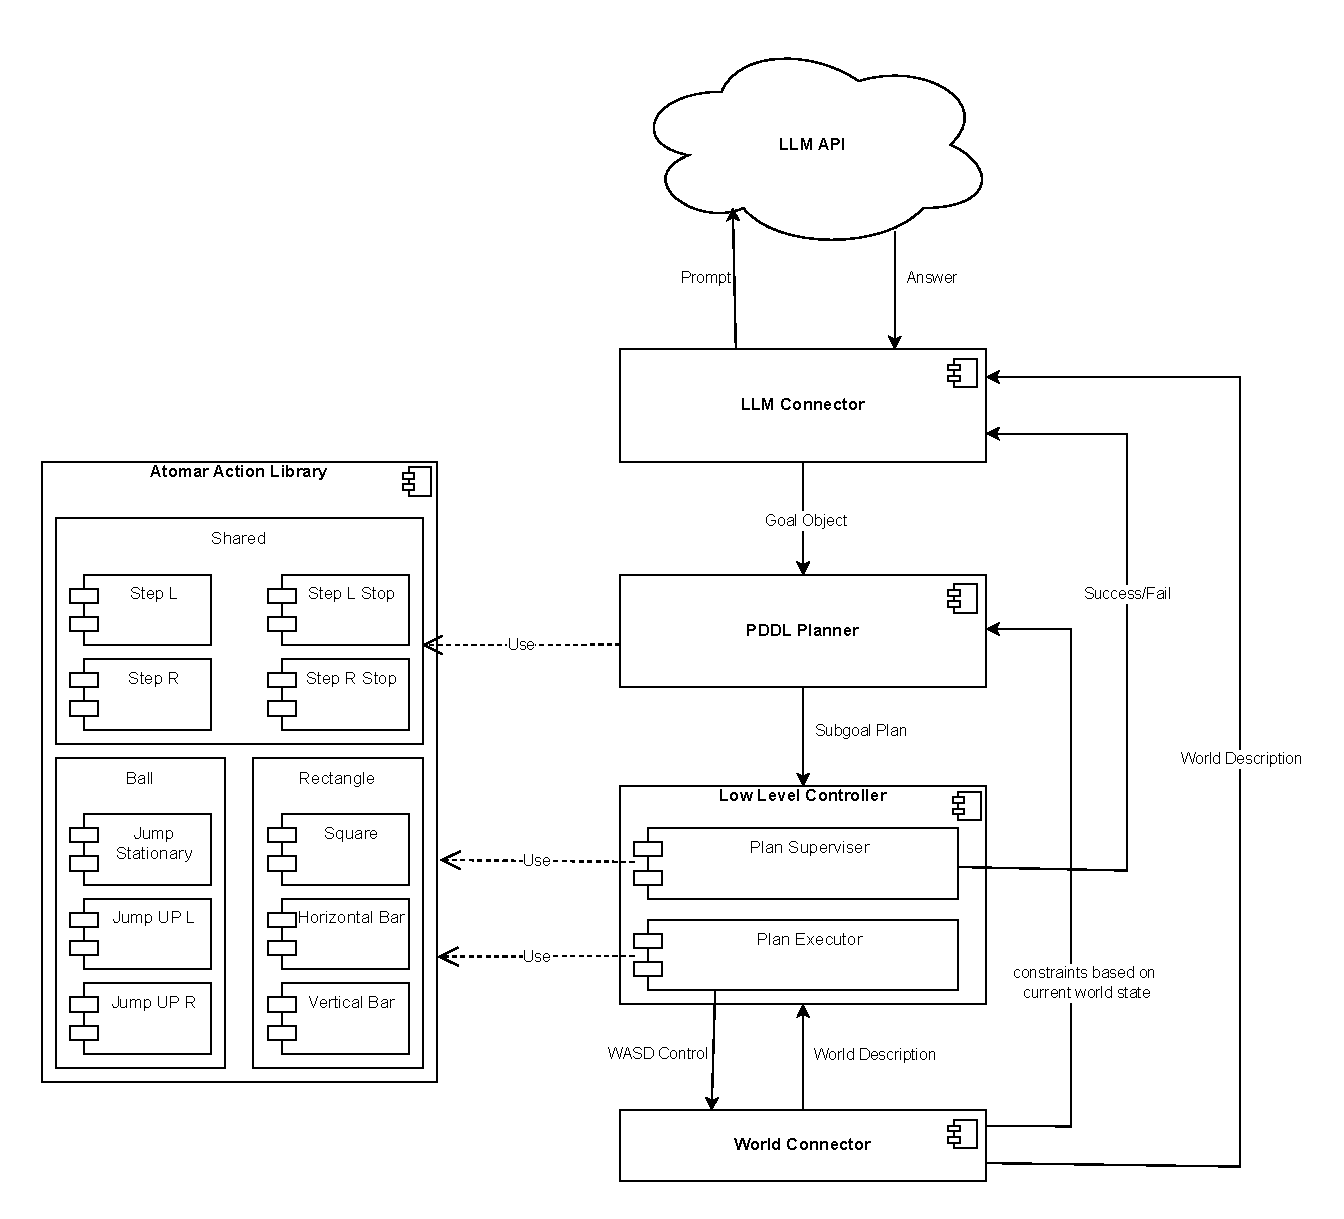
\includegraphics[width=0.7\textwidth]{graphic/IA_llm_agent.pdf}
\end{figure}

\section{Multi-Level planning with LLMs and traditional planning systems}

As inference on modern LLMs in computationally heavy and therefore causes high reaction latency to world changes, we task the LLM to find a sub-goal suitable to pursue in the current situation and a traditional planning system finds a sequence of atomic actions that lead to the sub-goal from the current situation. The LLM therefore acts similar to lifted online planning while the planner outputs a complete action sequence for reaching the next sub-goal, acting as a grounded planner. A success or fail of the plan as well as the executed actions and new world state are reported to the LLM by including them in the next prompt. The effect of selecting the last goal and the steps that where used in an attempt to reach it are therefore present in the input data and can be considered when choosing the next sub-goal.

\section{Low level planning with traditional planner}

To prepare the world description retrieved from the world connector for usage with a planner, it has to be converted to a discrete state space. Like in exercise 12 of the practicals, a rasterization is applied to model the planning problem in PDDL and use an automated planner. A domain file is created from the actions available for the current player type and their preconditions and effects. A problem file is created from the rasterized world description and the goal set by the LLM. The generated PPDL files are then fed to a planning system that delivers an action chain for the low level controller.

\section{Learning through LLM in-context learning}
% TODO Martin, Mohammad
%As already briefly explained in the general agent concept, a state of the art large language model is used as a versatile learning element to ...  %TODO to complete with the details that are currently in the organisation section
\section{Learning through LLM in-context learning}
As already briefly explained in the general agent concept, a state-of-the-art large language model (LLM) is used as a versatile learning element 
to dynamically adapt to the game environment. 
The LLM is not explicitly fine-tuned on the game itself but leverages its pre-trained knowledge and in-context learning capabilities 
to improve decision-making over time. Instead of relying on conventional reinforcement learning, 
which requires extensive training data and rewards, the LLM refines its planning through repeated interactions and contextual updates.

\subsection{Adaptive Decision-Making through In-Context Learning}
In-context learning enables the LLM to adjust its responses dynamically without modifying its weights. 
By providing structured prompts that include historical observations, world states, and agent actions, 
the LLM can iteratively refine its goal-setting and decision-making. 
This method allows the agent to leverage accumulated experience while maintaining adaptability to new situations. 
The interaction loop between the LLM and the planning module ensures that goal selection is continuously improved based on past successes and failures.

\subsection{Integration with PDDL for Logical Planning}
To ensure deterministic and efficient planning, the LLM-generated sub-goals are integrated with a Planning Domain Definition Language (PDDL)-based planner. 
The PDDL framework provides a structured representation of the environment, encoding available actions, their preconditions, and effects. 
The agent translates high-level LLM recommendations into PDDL problem files,
which are then processed by a planner to generate precise, executable action sequences.
By leveraging PDDL, the system mitigates LLM hallucinations, ensuring that proposed actions adhere to logical constraints. 
The generated plans undergo verification, with execution monitored for deviations that may necessitate replanning. 
This hybrid approach allows the agent to combine the adaptability of LLM-based goal selection with the structured precision of symbolic planning.

\subsection{Learning from Failures and Continuous Refinement}
To enhance decision-making efficiency, the agent systematically tracks failed plans and adapts subsequent goal-setting accordingly. 
If a generated plan fails due to unexpected environmental changes or incorrect assumptions, 
the failure is reported back to the LLM along with an updated world state. 
This enables the agent to avoid repeating past mistakes and gradually refine its strategy over multiple game runs.
By integrating in-context learning with symbolic planning, the agent achieves a balance between flexibility and determinism. 
This iterative learning process ensures continual improvement in planning efficiency, adaptability to dynamic environments, 
and better coordination in multi-agent interactions.

\section{Collaboration}

For complex collaboration with a shared plan with joint actions, a predefined communication interface would be needed. 
Only by communication of abilities and intention a common ground for strong collaboration could be found. 
Because of the scoring system the players are also in mild competition with each other, requiring negotiation over a communication interface to reach a common ground for a joint plan.  
As such an interface is not available, our agent has to rely on hints and creating a theory of mind model of the other agent. 
On its own, our agent will only select diamonds as goals and do not offer cooperation. The other player will however be considered in Planning and will be reported to the LLM. If the position of another agent gets considered useful for collecting a goal it can get used. As the sequence and history of perceptions of the other agent is also included in the prompt, we hope that the LLM will learn a model of the behaviour of the other agent by exploiting the theory of mind abilities of LLMs discussed in the lecture.

\section{Agent Evaluation}

To evaluate the implementation of our concept a series of experiments is conducted.
The first is the ability of the agent to deal with a new situation based only on the background knowledge provided by the prompt and LLM. For this a clean run (with new LLM chat) in levels of different complexity is conducted.
Possible levels are flat platforms with easily reachable diamonds as simple levels and levels with unrecoverable falls and unreachable diamonds on hard levels. 

To introduce a measure for the performance, the overall score of the controlled player is evaluated for the different levels.
Higher scores indicate a better understanding of the structure of the level, own abilities and other agent behaviour.
Also the number of required re-plannings while reaching a goal is measured. High values here indicate uncertainty in world and other player understanding. A re-planning occurs in a goal set by the LLM is not reachable or the execution of a plan gets interrupted by an execution failure (e. G. dropping in an undesired unrecoverable state) or a change of an object in the world that is part of the plan (e. G. target diamond gets collected).

To evaluate the learning ability of our agent we pick levels that our agent struggled with in the first try. Struggling is indicated by a low score and/or a high number of re-plannings. By letting the agent play the level with the knowledge about past goals and plan failures in the history and tracking the score and number of re-plannings over the rounds we evaluate the learning ability of our concept.

\section{Organization}

The Project can be split up in different work packets that can be worked on individually.
Ideas that emerged during discussions in the group are captured here. This causes different grades of detail for the different topics.

\subsection{Software Architecture}
To make the different components of the system work together, a software architecture and a framework defining the structure and communication of the application and the different components has to be defined. 
The logic and behaviour of the different components will then be added in this framework. 
The goal of this work package is a working python framework with callbacks for communication between the modules and defined interfaces. 
It will also include Communication with the simulation via the World connector.
As integration of the other functionality depends on this task, it has to be worked on early on.

\subsection{Self Localization}

This work package includes the implementation of the self localization mechanism described the agent description above. As the game application currently delivers information about the controlled player to the agent and the self localization module is independent from the main agent code this task can be worked on in the later development process or can be implemented in parallel to the other tasks. 

\subsection{Low Level Control}
The goal of this work package is the creation of a library of atomic actions for the disc and rectangle player. 
As the physics parameters of the game are not known, the actions will be implemented in a approximate way and return if the post-condition is met with a margin of error. 
It will also include a plan executor that will run an action sequence and check for success or fail.
A draft of preconditions and effects of the atomic actions for later use in the planning system is also included.

\subsection{Connect Planner to World and Actions}

This work package contains the development of a conversion routine from the world description from the world connector to a problem file. Also the final definition of available actions for the domain file based on the drafts from the low level control work package is included. 
A suitable planner for the generated files is then selected.

\subsection{LLM Setup and Provider Selection}
% TODO Martin, Mohammad
% only include setup and provider selection here as Prompt design and in contect learning is already tackled in agent desctiption

Since the agent runs on hardware with limited GPU resources, we rely on a remote API for the LLM. The chosen provider (e.g., Google Gemini) is expected to meet our usage constraints—less than 15 requests per minute (RPM), fewer than 1 million tokens per minute (TPM), and under 1,500 requests per day (RPD).


\textbf{API Setup:}
\begin{itemize}
    \item \textbf{Provider Selection:}  
    The LLM is accessed through a remote API, ensuring that our agent can perform advanced reasoning without requiring local GPU resources.
    
    \item \textbf{Connection and Authentication:}  
    Secure connections are established to the API endpoint, with proper authentication protocols in place. Rate limiting and error-handling procedures are also implemented to handle potential network issues or API downtimes.
    
    \item \textbf{Scalability Considerations:}  
    Given our relatively low usage expectations, the API configuration is optimized to maintain low latency while ensuring that each prompt-response cycle is efficient.
\end{itemize}


\begin{comment}
\textbf{Prompt Design:}
\begin{itemize}
    \item \textbf{Compact World Representation:}  
    The prompt is designed to provide the LLM with a concise yet informative snapshot of the current game state. This includes:
    \begin{itemize}
        \item The agent’s current position and status.
        \item The state and location of nearby objects (e.g., diamonds, traps).
        \item Observations regarding the other agent’s behavior.
        \item A summary of the recent action history and outcomes.
    \end{itemize}
    
    \item \textbf{Clear Instruction for Subgoal Selection:}  
    The prompt explicitly instructs the LLM to analyze the current state and propose a new subgoal. The instruction emphasizes criteria such as avoiding conflict with the other agent and selecting a subgoal that is viable given the current environmental conditions.
    
    \item \textbf{Dynamic Context Injection:}  
    A prompt template is used, wherein placeholders are dynamically populated with the latest world state and history data before sending the request. This helps the LLM leverage its in-context learning capabilities and develop a rudimentary theory of mind regarding the other agent.
    
    \item \textbf{Token Efficiency:}  
    To meet API limitations and ensure fast response times, the prompt is optimized to include only essential details.
\end{itemize}

A sample prompt template might look like this:

\begin{verbatim}
[World State]
- Agent Position: (x, y)
- Nearby Objects: [list with positions and statuses]
- Other Agent Observations: [brief summary of movements/actions]
- Recent Action History: [actions and outcomes]

Task: Based on the above state, determine the next viable subgoal that advances our overall objective while minimizing interference with the other agent.
\end{verbatim}

Once the prompt is sent to the LLM, the response is parsed to extract the recommended subgoal. This subgoal is then forwarded to the PDDL planner for generating the corresponding sequence of atomic actions, thereby closing the loop between high-level reasoning and low-level execution.

By combining a robust, remote LLM setup with a carefully designed prompt, our system leverages the flexible reasoning capabilities of the LLM while maintaining deterministic control through grounded planning.
\end{comment}


\subsection{Evaluation}
This work package includes the design of evaluation levels of different difficulty as well as running the experiments described in the agent evaluation section. As it requires a functional agent, it is the last task to be worked on in the project.

\subsection{Deployment}
The Goal of this work package is the creation of the final deliverable, a fully working docker container containing the agent. 
This task will be tackled by the group when the agent is working as a standalone application.


\end{document}
